\documentclass{emulateapj}

\usepackage{epsfig}
\usepackage{amsmath}
\usepackage{rotating}
\usepackage{natbib}
%\usepackage{lscape}
\usepackage{enumerate}
\usepackage{multirow}
\usepackage{array}
\usepackage{appendix}
\usepackage{comment}
\usepackage{color}
%\usepackage[dvipdfmx]{color}
%\usepackage[dvipdfmx]{graphicx}

% trivial change as a test

\bibliographystyle{apj}

\def\memoYF#1{\color{red}$[${\bf #1}$]$ \color{black}}

\def\memoDS#1{\color{blue}$[${\bf #1}$]$ \color{black}}

\def\plotonesc#1{\centering \leavevmode
\includegraphics[clip=, width=1.70\columnwidth]{#1}}
\def\plotoneh#1{\centering \leavevmode
\includegraphics[clip=, width=.95\columnwidth]{#1}}
\def\plotone#1{\centering \leavevmode
\includegraphics[clip=, width=.85\columnwidth]{#1}}
\def\plotoneShrinkSmall#1{\centering \leavevmode
\includegraphics[clip=, width=.49\columnwidth]{#1}}
\def\plotoneShrinkMed#1{\centering \leavevmode
\includegraphics[clip=, width=.55\columnwidth]{#1}}
\def\plotoneShrinkBig#1{\centering \leavevmode
\includegraphics[clip=, width=.65\columnwidth]{#1}}
\def\plottwo#1#2{\centering \leavevmode
\includegraphics[width=.45\columnwidth]{#1} \hfil
\includegraphics[width=.45\columnwidth]{#2}}
\def\plottwob#1#2{\centering \leavevmode
\includegraphics[width=.49\columnwidth]{#1} \hfil
\includegraphics[width=.49\columnwidth]{#2}}
\def\plottwor#1#2{\centering \leavevmode
\includegraphics[width=.55\columnwidth,angle=90]{#1} \hfil
\includegraphics[width=.55\columnwidth,angle=90]{#2}}
\def\plotthree#1#2#3{\centering \leavevmode
\includegraphics[width=.3\columnwidth]{#1} \hfil
\includegraphics[width=.3\columnwidth]{#2} \hfil
\includegraphics[width=.3\columnwidth]{#3}}

\newcommand{\cN}[1]{\mathcal{N}}
\newcommand{\pn}[1]{\mbox{$(#1)$}}
\newcommand{\spa}{\mbox{ }}
\def\gsim{\;\rlap{\lower 2.5pt
 \hbox{$\sim$}}\raise 1.5pt\hbox{$>$}\;}
\def\lsim{\;\rlap{\lower 2.5pt
   \hbox{$\sim$}}\raise 1.5pt\hbox{$<$}\;}

% set formatting properties
\setlength{\textwidth}{6.5in}
\setlength{\textheight}{8.8in}
\setlength{\hoffset}{0.0in}
\setlength{\voffset}{-0.4in}
%\setlength{\voffset}{0.3in}
\parindent 0.2in
\parskip 0.1in



%%%%%%%%%%%%%%%%%%%%%%%%%%%%%%%%%%%%%%%%%%%%%%%%%
% THE DOCUMENT BEGINS HERE                      %
%%%%%%%%%%%%%%%%%%%%%%%%%%%%%%%%%%%%%%%%%%%%%%%%%

%\slugcomment{Submitted to ApJ, 20 October 2011}

\begin{document}


%%% Begin front material
%\twocolumn[%%% Begin front material

\title{Red-Giant Hot Jupiters: Brilliant Radio Beacons?}

\author{
%
Yuka Fujii\altaffilmark{0} \\
%
David S. Spiegel\altaffilmark{1, 2} \\
%
{\bf and some order:} \\
%
Jason Nordhaus\altaffilmark{3} \\
%
Nikku Madhusudhan\altaffilmark{4} \\
%
Mehrdad Mirbabayi\altaffilmark{1} \\
%
Aaron Parsons\altaffilmark{4} \\
%
Tony Mroczkowski\altaffilmark{5,6} \\
%
Neil Zimmerman\altaffilmark{7}
}

\affil{$^0$Earth-Life Science Institute, Tokyo Institute of Technology, 
  Tokyo, JAPAN, 152-8550}
  
\affil{$^1$Astrophysics Department, Institute for Advanced Study,
  Princeton, NJ 08540}

\affil{$^2$Research \& Development, Sum Labs,
  New York, NY  10001}

\affil{$^2$Department of Mathematics, Rochester Institute of Technology}

\affil{$^3$Astronomy Department, University of Cambridge, UK}

\affil{$^4$Astronomy Department, University of California Berkeley}

\affil{$^5$National Research Council Fellow}

\affil{$^6$Naval Research Laboratory, 4555 Overlook Ave SW, Washington, DC 20375}

\affil{$^7$Department of Mechanical and Aerospace Engineering, Princeton University, Princeton, NJ 08544}


\vspace{0.5\baselineskip}

\email{
yuka.fujii@elsi.jp
}


\begin{abstract}
%%%
Magnetized planets emit radio wave in the interaction with stellar wind. 
When the host stars evolve off the main sequence and go through red-giant branch (RGB), the stars become orders-of-magnitudes more luminous and at the same time lose mass at much higher rate than their main-sequence counterparts. 
Accordingly, planetary companions around them at a few AU orbits, if exist, are heated up to the level of canonical hot Jupiters and also subjected to the massive stellar wind. 
Such ``Red-Giant Hot Jupiters'' (RGHJs) are therefore candidates of bright radio emitters. 
We estimate the spectral auroral radio intensity of RGHJs employing the ``radio Bode's law'' and proposed scaling of planetary magnetic fields. 
We find that RGHJs would be as bright as the predicted radio emission from canonical hot Jupiters, and can be even brighter depending on the configurations. Thus radio emission from a RGHJ might be visible from a hundred parsec distances with current/future detectors \memoYF{check}. 


%Red-giant hot Jupiters (RGHJs) are jovian planets orbiting red-giant-branch (RGB) or asymptotic-giant-branch (AGB) stars. 
%Red-giant hot Jupiters (RGHJs) are jovian planets orbiting red-giant-branch (RGB) or asymptotic-giant-branch (AGB) stars.
%Post-main-sequence stars lose mass at much higher rates than main-sequence stars.
%A jovian planet passing through the dense winds of its RGB or AGB host can capture stellar wind in its magnetosphere, leading to radio emission from electrons spiraling in the magnetic field.
%The cyclotron frequency of electrons from the stellar wind accreting onto the planet scales as 100~MHz~$(B/30 {\rm~Gauss})$.
%The cyclotron frequency of electrons from the stellar wind accreting onto the planet scales as 100~MHz~$(B/30 {\rm~Gauss})$.
%Counterintuitively, a plausible toy model suggests that a stronger planetary magnetic field leads to lower spectral flux density, and might therefore make objects more challenging to observe.
%Still, for a range of planetary and stellar parameters, a RGHJ might generate a radio luminosity that would be visible from kiloparsec distances.
\end{abstract}


\keywords{planets and satellites: Jupiter --- Sun: evolution ---
  planetary systems --- stars: evolution ---
  stars: AGB and post-AGB}
%]%%% End front material


%%%%%%%%%%%%%%%%%%%%%%%%%%%%%%%%%%%%%%%%%%%%%%%%%%%%%%%%%%%%%%%%%%%
\section{Introduction}
\label{sec:intro}
%%%%%%%%%%%%%%%%%%%%%%%%%%%%%%%%%%%%%%%%%%%%%%%%%%%%%%%%%%%%%%%%%%%


Planets with strong magnetic fields may generate radio or X-ray emission when interacting with energetic charged particles. 
It has been known that Jupiter emits radio emission from the radiation belt and auroral region due to cyclotron-maser instability \citep{zarka1998}.  % due to the acceleration of the plasmas. \memoYF{?}.
Potentially, exoplanets can also emit radio waves through the similar mechanisms, depending on their intrinsic magnetic fields and the density of surrounding plasmas, e.g. stellar wind particles and particles from Io-like moons. 
Observations of radio emission from Solar System planets imply an empirical relation that the radio intensity is proportional to the input solar wind flux going into each planetary magnetosphere, which is known as  ``radiometric Bode's law'' \citep{desch+kaiser1984}. 
Based on this law, exoplanets in close-in orbits have been attracted attention as possible bright radio wave emitters because they are subjected to strong stellar wind and/or strong interstellar magnetic field, and thus can gain larger energy input. Motivated by such speculations, spectral radio intensity from known exoplanets have been estimated  \citep{farrell1999,zarka2001,Lazio2004,griesmeier2004,griesmeier2007a,griesmeier2007b,reiners2010}. 
In addition, young planetary systems where the stellar wind activity is stronger are also taken into consideration \citep{griesmeier2005}. 
Although the observational search for these radio signatures are being conducted, there is no clear detection claimed so far
\citep{bastian2000,george2007,stroe2012,hallinan2013,murphy2015}, 
while some indications have been obtained \citep{lecavelier_et_al2013,sirothia2014}. 

When stars less than $\sim$8~$M_\sun$ evolve off the main sequence,
they go through stages on the red-giant branch (RGB) and the
asymptotic-giant branch (AGB) where their radii and luminosities increase by orders of magnitude. 
Jovian planets in orbit around such stars can be transiently heated to hot-Jupiter temperatures ($\sim$1000~K or more) at distances out to tens of AU, depending on the star's mass \citep{spiegel+madhusudhan2012}. 
At the same time, they are subject to massive (but slow) stellar wind, as the mass-loss rate of such evolved stars are significantly higher than the main-sequence counterparts, ranging from $\sim  10^{-8} M_\odot$/yr to $\sim  10^{-5} M_\odot$/yr with the highest values for AGB stars \citep[e.g.,][]{reimers1975, schild1989, vassiliadis1993, schoier2001, vanloon2005}, significantly larger than solar mass-loss rate $\sim 10^{-14}M_\odot$/yr. 
On the assumption that the radio emission is correlated with the stellar wind, planetary companions around evolved stars could also generate bright radio emission. 

In this paper we estimate the potential to detect planetary companions around evolved stars through the brightness of their radio emission. 
In \S2, we describe our assumptions for the scaling of planetary radio emission, stellar wind, and planetary magnetosphere.
\S3 presents a simple estimate of the spectral radio intensity of RGHJs and compares them with what might be expected from canonical hot Jupiters.
%\S3 also describes the surprising result that, although the planetary magnetic field is crucial to the generation of radio emission at all, there might be an important region in parameter space in which planets with stronger magnetic fields are less easily observable. 
\S4 discusses possible obstacles to detect radio emission from RGHJs, in particular the effects of intrinsic radio emission of evolved stars and the offsetting effect of the electrons spiraling down along the planetary magnetic field.
Observability with current and near-future instruments is also examined in \S4. 
Finally, \S5 concludes the paper with a brief summary. 

%Roughly 20\% of the more than 700 \memoYF{check!} currently known exoplanets around main-sequence stars \footnote{See online catalogs such as http://www.openexoplanetcatalogue.com/ \citep{rein2012}, http://exoplanet.eu \citep{schneider_et_al2011}, or http://exoplanets.org \citep{wright_et_al2011} for up-to-date lists.} have masses greater than half of Jupiter's, orbital radii greater than 1~AU, and will become hot Jupiters (i.e., for the present purposes, this means they will receive at least as much irradiation as the currently known hot Jupiters/Neptunes \citep{spiegel+madhusudhan2012}. 


%%%%%%%%%%%%%%%%%%%%%%%%%%%%%%%%%%%%%%%%%%%%%%%%%%%%%%%%%%%%%%%%%%%
\section{Model}
\label{s:assumptions}
%%%%%%%%%%%%%%%%%%%%%%%%%%%%%%%%%%%%%%%%%%%%%%%%%%%%%%%%%%%%%%%%%%%

\memoYF{In the end the number of significant decimal digits is set to 1 or 2.}

Before estimating the frequency of planetary radio emission and the spectral radio intensity, we specify the property of the stellar wind of the evolved stars in \S\ref{ss:stellarwind}, and that of planetary magnetic field in \S\ref{ss:magneticfield}.  
Then, we discuss the framework to estimate the frequency and intensity of planetary radio emission in \S\ref{ss:model_frequency} and \S\ref{ss:model_intensity}, respectively. 



%%%%%%%%%%%%%%%%%%%%%%%%%%%%%%%%%%%%%%%%%%%%%%%%%%%%%%%%%%%%%%%%%%%
\subsection{Assumptions for Stellar Wind}
\label{ss:stellarwind}
%%%%%%%%%%%%%%%%%%%%%%%%%%%%%%%%%%%%%%%%%%%%%%%%%%%%%%%%%%%%%%%%%%%

One important factor in modeling the radio emission due to the interaction with stellar wind and the planetary magnetic field is the density and velocity of stellar wind. 
The number density of stellar wind, $n$, can be expressed as
%%%%%%%%%% 
\begin{equation}
n = \frac{\dot M_\star}{4\pi a^2 m_p v}
\label{eq:n}
\end{equation}
%%%%%%%%%% 
where $\dot M_\star$ is the stellar mass loss rate, $a$ is the orbital distance from the star and $m_p$ is proton mass, and $v$ is the velocity of the stellar wind. 

While the solar mass loss rate, $\dot M_\odot$, is $\dot M_\odot \sim 2\times 10^{-14} M_{\odot}$/yr \citep[e.g.,][]{hundhausen1997}, the mass loss rate of red giants is typically $\dot M_\star \sim 10^{-8}-10^{-7} M_{\odot}$/yr, ant the rate can be as high as $10^{-5} M_\odot{\rm /yr}$ during the AGB phase. 
Therefore, we have
%%%%%%%%%% 
\begin{equation}
\frac{\dot M_\star}{\dot M_{\odot}} \sim 10^6 - 10^9
\end{equation}
%%%%%%%%%% 

On the other hand, the stellar wind velocity becomes smaller because of the small escape velocity (due to expanded stellar radius).
%\footnote{Escape velocity is $\sqrt{2GM/r}$.}
Assuming that the stellar wind scales as the escape velocity, i.e., $\propto \sqrt{2GM_p/R}$ ($G$ is the gravitational constant, $M_p$ is the planetary mass, and $R$ is the planetary radius), a RG with radius $R=100R_{\odot}$ has 10 times as slow stellar wind as that at the main sequence. 
%\memoYF{Estimate in more detail?} 
Thus, 
\begin{equation}
\frac{v}{v_{\odot}} \sim 10^{-1}
\end{equation}
where $v_{\odot} \sim 4.0 \times 10^2 $ km/sec. 

%The temperature of stellar wind of RGs is expected to be 2 orders of magnitude lower than their main sequence counterparts, mainly because the sound speed of hot corona exceeds the escape speed, i.e., hot corona cannot be confined in the stellar atmosphere \citep{suzuki2008}. 
%\begin{equation}
%\frac{T}{T_{\odot}} \sim 10^{-2}
%\end{equation}
%where $T_{\odot } \sim 10^6$ K. 

%%%%%%%%%%%%%%%%%%%%%%%%%%%%%%%%%%%%%%%%%%%%%%%%%%%%%%%%%%%%%%%%%%%
\subsection{Assumptions for Planetary Magnetic Field}
\label{ss:magneticfield}
%%%%%%%%%%%%%%%%%%%%%%%%%%%%%%%%%%%%%%%%%%%%%%%%%%%%%%%%%%%%%%%%%%%

In order to estimate the planetary magnetic field of general planets, we adopt a simple scaling relation between the magnetic field and macroscopic planetary properties. 

Several relationships have been proposed so far \citep[e.g.][]{russel1978,busse1976,stevenson1979,mizutani1992,sano1993,starchenko2002,christensen2006} %\memoYF{check!}
(see \citet{griesmeier2004} or \citet{christensen2010} for the summary), which are compared with numerical simulations in \citet{christensen2010}. 
We employ the following relationship from \citet{christensen2006}, which is based on the assumption that the ohmic dissipation energy is a fraction of available convected energy and was found to be in a good agreement with the numerical experiments over a wide parameter space: 
%\memoYF{describe in more detail}:
%%%%%%%%%% 
\begin{equation}
B^2 \propto \rho_c r_c^{4/3} q_c^{2/3}, \label{eq:Bscaling} 
\end{equation}
%%%%%%%%%%
where $\rho _c$ and $r_c$ are the density and the radius of the dynamo region, and $q_c$ is the internal convected energy flux in the core region. 
Magnetic field of planets are estimated by scaling Jovian magnetic field $B_J \sim 10$~G by equation (\ref{eq:Bscaling}). 
\memoYF{need to cite \citet{reiners2010} somewhere.}

In order to evaluate $\rho _c $ and $r_c$, we need a model of internal structure of planets. 
In this paper, we consider Jupiter-like gaseous planets and assume that the planetary radius is constant at $R_p = R_{p,J}$, because the numerical calculations show that the radii of gaseous planets over the range of $0.1 M_{p, J} < M_p < 10M_{p, J}$ (with core mass less than 10\%) are converged to $0.8 R_{p, J} < R_p < 1.2R_{p, J}$ within 1 Gyr \citep{fortney2007}. 
For the density profile, we assume a polytrope gas sphere with index $n=1$, which results in:
%%%%%%%%%% 
\begin{equation}
\rho [r] = \left( \frac{\pi M_p}{4 R_p^3} \right) \frac{\sin \left[ \pi \frac{r}{R_p} \right]}{\left( \pi \frac{r}{R_p} \right)}. \label{eq:rho_r}
\end{equation}
%%%%%%%%%%
We determine the core radius $r_c$ by assuming that the hydrogen becomes metallic when $\rho (r)$ exceeds the critical density $\rho_{\rm crit}=0.7\,\mbox{g/cm}^3$ \citep{exoplanets2006, griesmeier2007b}. The density of the metallic core, $\rho _c$ is obtained by averaging the density in the core. 
In the case of Jupiter, $r_{c,\,J} = 0.85 R_{\rm J}$.  

The scaling of convected heat flux, $q_c$, is obtained by dividing the time-dependent net planetary luminosity by the surface area of the core region i.e., $4\pi r_c^2$. 
The model of luminosity evolution is taken from \citet{burrows_et_al2001} \citep[see also][]{marley2007}, which resulted in:
%%%%%%%%%%
\begin{equation}
L \sim 1.4^{-9} L_\odot \left( \frac{t}{4.5 \rm~Gyr} \right)^{-1.3} \left( \frac{M_p}{M_J} \right)^{2.64} \, 	
\label{eq:burrowsLum}
\end{equation}
%%%%%%%%%%
Therefore, we have
%%%%%%%%%%
\begin{equation}
q_c \sim q_{c, J} \left( \frac{t}{4.5 \rm~Gyr} \right)^{-1.3} \left( \frac{M_p}{M_J} \right)^{2.64} \left( \frac{r_c}{r_{c,\,J}} \right)^{-2}\, .
\label{eq:burrowsHeatFlux}
\end{equation}
%%%%%%%%%%
%We estimate the convected heat flux by dividing this luminosity by the surface area of the core region, i.e., $4 \pi r_c^2$. 

%\memoYF{I am not sure if the following paragraph is needed.}
%There also exist several other scaling relations proposed so far, which is compared in \citet{christensen2010}. 
%In particular, \citet{griesmeier2004} estimated radio emission of discovered exoplanets based on the following scaling relationship: 
%%%%%%%%%% 
%\begin{equation}
%\mathcal{M} \propto  \omega ^{\alpha } \rho_c ^{\beta } r_c^{\gamma } \sigma ^{\delta }
%\end{equation}
%%%%%%%%%%
%where $\omega $ is the spin angular velocity and $\sigma $ is the conductivity of the ``dynamo region'', which is assumed to be same as Jupiter. 
%The scaling indexes are estimated to be $\alpha \sim 1/2-1$, $\beta \sim 1/2$, $\gamma \sim 3-4$, and $\sigma \sim -1/2-0$. 
%
%Unlike canonical hot jupiters, RGHJs are not subject to tidal lock, as the gravitational effects of their host star does not change even if the star evolves into red giants. Without no physical insights of the typical spin rate, we could assume that of Jupiter: $\omega = 9.925$ [hr]. 

%%%%%%%%%%%%%%%%%%%%%%%%%%%%%%%%%%%%%%%%%%%%%%%%%%%%%%%%%%%%%%%%%%%
%\subsection{Cut-off frequency}
%\label{ss:cutoff}
%%%%%%%%%%%%%%%%%%%%%%%%%%%%%%%%%%%%%%%%%%%%%%%%%%%%%%%%%%%%%%%%%%%


%%%%%%%%%%%%%%%%%%%%%%%%%%%%%%%%%%%%%%%%%%%%%%%%%%%%%%%%%%%%%%%%%%%
\subsection{Frequency of Radio Emission}
\label{ss:model_frequency}
%%%%%%%%%%%%%%%%%%%%%%%%%%%%%%%%%%%%%%%%%%%%%%%%%%%%%%%%%%%%%%%%%%%

The peak of the auroral radio emission is around the cyclotron frequency of the planetary magnetic field, $f_{\rm cyc}$: 
%%%%%%%%%% 
\begin{equation}
f_{\rm cyc} = \frac{eB}{2\pi m_e} \approx 27.9 {\rm~MHz} \left( \frac{B}{10 \rm~G} \right) \label{eq:fcyc}
\end{equation}
%%%%%%%%%%
where $e$ and $m_e$ are the charge and mass of the electron, respectively.

Radio emission from the planet is observable from ground only when the maximum frequency is larger than the plasma frequency of Earth's ionosphere $f_{\rm plasma}^\oplus$ and the maximum plasma frequency along the line of sight $f_{\rm plasma}^{\rm los}$.
The plasma frequency may be expressed as
\begin{eqnarray}
f_{\rm plasma} & = & \sqrt{\frac{n_e e^2}{\pi m_e}} \\
 & = & 8979 {\rm~Hz} \times \left( \frac{n_e}{\rm cm^{-3}} \right)^{1/2} \, .
\label{eq:fplasma}
\end{eqnarray}
In the Earth's ionosphere, the electron number density is less than $10^6$~cm$^{-3}$, which implies that $f_{\rm plasma}^\oplus \lsim 10$~MHz.
At the favorable viewing condition, when the planet is on the near side of its star to the Earth, the maximum plasma frequency along the line of sight corresponds to that in the vicinity of the planet.
Therefore, combining Eq.~(\ref{eq:n}) and Eq.~(\ref{eq:fplasma}), we have
%%%
\begin{eqnarray}
\label{eq:fplasmalos} f_{\rm plasma}^{\rm los} & \sim & 8.98 {\rm~kHz} \times \left( \frac{\dot M_\star}{4 \pi a^2 m_p v} \times 1\rm~cm^3 \right)^{1/2} \\
\label{eq:fplasmalos_scaled} & = & 14.7{\rm~MHz} \times \left( \frac{a}{5~\mbox{AU}}\right)^{-1} \left(\frac{v}{0.1 v_{\odot}}  \right)^{-1/2} \notag \\
 & & \times \left( \frac{\dot M_\star}{10^6 \dot M_{\odot}}\right)^{1/2} \, ,
\end{eqnarray}
%%%
where in Eq.~(\ref{eq:fplasmalos_scaled}) we have taken the solar mass-loss rate $\dot M_\odot$ to be $2.0 \times 10^{-14}~M_\odot$/yr and the typical solar wind velocity $v_{\odot }$ to be 400~km/sec.

%%%%%%%%%%%%%%%%%%%%%%%%%%%%%%%%%%%%%%%%%%%%%%%%%%%%%%%%%%%%%%%%%%%
\subsection{Flux of Radio Emission}
\label{ss:model_intensity}
%%%%%%%%%%%%%%%%%%%%%%%%%%%%%%%%%%%%%%%%%%%%%%%%%%%%%%%%%%%%%%%%%%%

The auroral radio spectral flux of exoplanets observed at the Earth, $F_{\nu}$ can be expressed by:
%%%
\begin{equation}
F_{\nu} = \frac{P_{\rm radio}}{\Omega l^2 \Delta f}
\label{eq:Fnu}
\end{equation}
%%%
where $P_{\rm radio}$ is the energy that is deposited as radio emission of considered frequency range, $\Omega $ is the solid angle of the emission, $l$ is the distance between the target and the Earth, and $\Delta f$ is frequency bandwidth. 

We estimate the radio emission of exoplanets, $P_{\rm radio}$, simply by scaling the Jovian auroral radio emission, $P_{\rm radio,\,J}$, with the input energy from stellar wind, in the same manner as \citet{griesmeier2005,griesmeier2007a,griesmeier2007b}. 
The scaling is based on the empirical/apparent good correlation between the radio emission intensity of Solar System planets and the input kinetic energy or the magnetic energy of the solar wind \citep[``radio Bode's law''; ][]{desch+kaiser1984}, i.e.,
%Namely, although the detail of the mechanism to generate planetary radio emission is not fully understood so far \memoYF{cite something?}, 
%observations indicate that the total radio emission, $P_{\rm radio}$ is proportional to the input kinetic energy, $P_{\rm k,\,inp}$, or the input magnetic energy, $P_{\rm m,\,inp}$ \citep[``radio Bode's law''; ][]{desch+kaiser1984}:
%%%
\begin{eqnarray}
P_{\rm radio} &\propto & P_{\rm inp} \\
P_{\rm inp,\,k} &=& n v^3 r_s ^2 \label{eq:Pinp_kin}, \\
P_{\rm inp,\,m} &=& v B_{\bot }^2 r_s ^2 \label{eq:Pinp_mag},
\end{eqnarray}
%%%
where $ B_{\bot }$ is the interstellar magnetic field perpendicular to the stellar wind flow, and $r_s$ is the radius of the magnetic stand-off point. 
%
In the case of the Solar wind, the kinetic energy is dominant input energy over the magnetic one (the former is $\sim 400$ times larger than the latter).  
It is not clear from the observations of the Solar System planets which is the fundamental one, the correlation to the input kinetic energy, that to the magnetic energy, or both. 


In this paper, we assume that the radio emission is scaled with the input kinetic energy, i.e., $P_{\rm radio} \propto P_{\rm k,\,inp}$, because as indicated earlier, the kinetic energy of the stellar wind of evolved stars are much larger than the main-sequence stars and thus may lead to brighter radio emission. 


On the other hand, if the correlation with input magnetic energy is more fundamental, it is difficult to estimate the planetary radio emission at this point because magnetic field of evolved stars are not well known for highly evolved stars; many of observations only set an upper limit \citep[e.g.,][]{konstantinova2010,petit2013,tsvetkova2013,konstantinova2013,auriere2015}. 
In the case of M-type giant EK boo, surface magnetic field $\sim 0.1-10 $G has been measured; In this particular case, given the large stellar radius $R_\star \sim 210 R_{\odot }$ the magnetic moment may be about $10^3$ times larger than the Sun and thus also may also increase the planetary radio emission. However, because of the lack of universal understanding of the stellar magnetic field, we leave the magnetic model of radio emission for evolved stars for future work. 

In reality, the total power of Jovian auroral emission highly varies in time: $1.3\times 10^{10}$ W for the average, $3.2\times 10^{10}$ W for the average of highly active time, and $4.5 \times 10^{11}$ W for the peak activity \citep{zarka_et_al2004}. Here we employ $P_{\rm radio,\,J}=2.1\times 10^{11}\mbox{~W}$ as a canonical value, following \citet{griesmeier2005,griesmeier2007b}.

The radius of the magnetic stand-off point, $r_s$, is obtained based on the balance between the stellar wind pressure and the planetary magnetic pressure: 
%%%
\begin{equation}
m_p n v ^2 \sim \frac{B^2}{8\pi}\left( \frac{r_s}{R_p} \right)^{-6}  \label{eq:stand-off}
\end{equation}
%%%
The radius obtained for Jupiter from this equality is about a half of actual radius of Magnetosphere \citep[][]{griesmeier2005}. We estimate $r_s$ simply by scaling Jovian magnetosphere \citep[$r_{s,\,J} \sim 84 R_J$][]{joy2002} according to equation (\ref{eq:stand-off}), i.e., 
%%%
\begin{eqnarray}
r_s 
%&\sim & R_p \left( \frac{B^2}{8\pi m_{\rm p}nv^2} \right)^{1/6}  \\
&=& r_{s,\,J} \left( \frac{B}{10~\mbox{G}} \right)^{1/3} \left( \frac{a}{5.2\mbox{AU}} \right)^{1/3}  \\
&& \times \left( \frac{\dot M_\star}{\dot M_\odot} \right)^{-1/6}  \left( \frac{\dot v}{v_{\odot }} \right)^{-1/6} \\
&=& 11.3 \, R_J \left( \frac{B}{10~\mbox{G}} \right)^{1/3}  \left( \frac{a}{5\mbox{AU}} \right)^{1/3} \\
&& \times \left( \frac{\dot M_\star}{10^6 \dot M_\odot} \right)^{-1/6}  \left( \frac{\dot v}{10^{-1}v_{\odot }} \right)^{-1/6}
 \label{eq:stand-off-radius}
\end{eqnarray}
%%%

%Thus, the radio emission, $P_{\rm radio}$, or equivalently the input kinetic energy, $P_{\rm k,\,inp}$, are estimated with $n$, $v$, and $\mathcal{M}$, which should be specified by assuming the properties of the stellar wind and the planetary magnetic field. 
%In the following, we describe our assumptions for these properties. 

We assume that the solid angle of the emission is same as the Jupiter's one for all of the exoplanets. In reality, the solid angles of auroral radio emission from  Jupiter, Saturn, and Earth are $\sim 1.6$, $\sim $6.3, and $\sim $3.5, respectively \citep{desch+kaiser1984}, which are on the same order and will not significantly affect our order-of-magnitude estimate of radio emission. 

The bandwidth, $\Delta f$, is assumed to be proportional to the representative frequency of the emission, which is the cyclotron frequency, following the assumption of \citet{griesmeier2007b}.

%We estimate the radio brightness of RGHJs by simply scaling \memoDS{stray sentence fragment?}


%%%%%%%%%%%%%%%%%%%%%%%%%%%%%%%%%%%%%%%%%%%%%%%%%%%%%%%%%%%%%%%%%%%
\section{Results}
\label{s:result}
%%%%%%%%%%%%%%%%%%%%%%%%%%%%%%%%%%%%%%%%%%%%%%%%%%%%%%%%%%%%%%%%%%%

%%%%%%%%%%%%%%%%%%%%%%%%%%%%%%%%%%%%%%%%%%%%%%%%%%%%%%%%%%%%%%%%%%%
\subsection{Estimate of Planetary Magnetic Field and Maximum Frequency}
\label{ss:Bplanet}
%%%%%%%%%%%%%%%%%%%%%%%%%%%%%%%%%%%%%%%%%%%%%%%%%%%%%%%%%%%%%%%%%%%s

First, we estimate the strength of planetary magnetic field based on the scaling relation of equation (\ref{eq:Bscaling}) and assumptions described in \S\ref{ss:magneticfield}. 
Figure \ref{fig:planetaryB} shows the estimated core radius ($r_c$), core density ($\rho_c$), and convected heat flux ($q_c$) as well as the predicted magnetic field strength at planetary surface ($B$) and the corresponding cyclotron frequency ($f_{\rm cyc}$), as functions of planetary mass and the age. 
Because $\rho _c \propto M_p$  at large $M_p$ and $q_c \propto t^{-1.3} M_p^{2.64}/r_c^2$, the magnetic field is roughly:
%%%%%%%%%% 
\begin{eqnarray}
B   &\sim &  10~{\rm G} \left( \frac{t}{4.5~\rm{Gyr}} \right)^{-0.43} \left( \frac{M_p }{M_{p,J}} \right)^{1.38} \label{eq:scalingB} \\
f_{\rm cyc} &\sim &  28~{\rm MHz} \left( \frac{t}{4.5~\rm{Gyr}} \right)^{-0.43} \left( \frac{M_p }{M_{p,J}} \right)^{1.38} \label{eq:scalingfc} 
\end{eqnarray}
%%%%%%%%%%
under this model. 

Note that the cyclotron frequency of Jovian planets older than 1~Gyr is typically larger than 10~MHz, the plasma cut-off frequency of Earth's ionosphere, and less than 1~GHz. 
In this regime, there are a number of current and near-future radio wave detectors including UTR-2, LOFAR, LWA, and SKA. 


%%%%%%%%%%%%%%%%%%%%%%%%%%%%%%%%%%%
\begin{figure}[htbp]
   \plotoneh{model_planetaryB_cgs.pdf}
   \caption{Planetary magnetic field as a function of age and planetary mass, based on the scaling of magnetic field of \citet{christensen2010} and the evolution of internal heat of \citet{burrows_et_al2001}.} %\memoDS{Can we change density to cgs in this figure?}
  \label{fig:planetaryB}
\end{figure}
%%%%%%%%%%%%%%%%%%%%%%%%%%%%%%%%%%% 




%%%%%%%%%%%%%%%%%%%%%%%%%%%%%%%%%%%%%%%%%%%%%%%%%%%%%%%%%%%%%%%%%%%
\subsection{Estimate of Radio Intensity of RGHJs in comparison with canonical HJs}
\label{ss:brightness}
%%%%%%%%%%%%%%%%%%%%%%%%%%%%%%%%%%%%%%%%%%%%%%%%%%%%%%%%%%%%%%%%%%%

Based on the assumption that the radio emission is proportional to the input kinetic energy (equation \ref{eq:Pinp_kin}), the scaling of the radio emission is expanded as follows:
%%%
\begin{eqnarray}
P_{\rm k,\,inp} &=& nv^3 r_s^2 = n v^3 \left( \frac{B^2}{2\pi m_{\rm p}nv^2} \right)^{1/3}  \\
&=& P_{\rm k,\,inp,\,J} \left( \frac{B}{B_J} \right)^{2/3} \left( \frac{a}{5.20~\mbox{AU}} \right)^{-4/3}  \notag \\
&& \times \left( \frac{\dot M_\star}{\dot M_{\odot}} \right)^{2/3} \left( \frac{v}{v_{\odot}} \right)^{5/3} \label{eq:Pkinp}
\end{eqnarray}
%%%

Now, we compare radio emission power of canonical hot Jupiters and that of red giant hot Jupiters.
Canonical values we adopt for planetary mass, orbital distance, and orbital period of each type as shown in Table \ref{tab:comp_HJ}.
Then, equation (\ref{eq:Pkinp}) can be re-normalized as follows.
%%%
\begin{eqnarray}
P_{\rm k,\,inp} 
&\approx & 227 ~P_{\rm k,\,inp,\,J} \left( \frac{B}{B_J} \right)^{2/3} \left( \frac{a}{5~\mbox{AU}} \right)^{-4/3} \notag \\
&& \times \left( \frac{\dot M_\star}{10^6 \dot M_{\odot}} \right)^{2/3} \left( \frac{v}{10^{-1} v_{\odot}} \right)^{5/3} \\
&& \;\;\;\;\;\;\;\;\;\;\;\;\;\;\;\;\;\;\;\;\; \mbox{(for RGB stars' companions)} \notag \\
&\approx & 2.27 \times 10^4 ~P_{\rm k,\,inp,\,J} \left( \frac{B}{B_J} \right)^{2/3} \left( \frac{a}{5~\mbox{AU}} \right)^{-4/3} \notag \\
&& \times \left( \frac{\dot M_\star}{10^9 \dot M_{\odot}} \right)^{2/3} \left( \frac{v}{10^{-1} v_{\odot}} \right)^{5/3}  \\
&& \;\;\;\;\;\;\;\;\;\;\;\;\;\;\;\;\;\;\;\;\; \mbox{(for AGB stars' companions)} \notag \\
&\approx & 489 ~P_{\rm k,\,inp,\,J} \left( \frac{B}{B_J} \right)^{2/3} \left( \frac{a}{0.05~\mbox{AU}} \right)^{-4/3} \notag \\
&& \times \left( \frac{\dot M_\star}{\dot M_{\odot}} \right)^{2/3} \left( \frac{v}{v_{\odot}} \right)^{5/3} \\
&& \;\;\;\;\;\;\;\;\;\;\;\;\;\;\;\;\;\;\;\;\; \mbox{(for canonical hot jupiters)} \notag 
\end{eqnarray}
%%%
Here, we normalized the strength of magnetic field of canonical hot jupiters with $B_J$, due to the uncertainty of the magnetic field of tidally-locked planets. 
Depending on the modeling of magnetic field strength, there is also a speculation that the tidally-locked planets may have weaker magnetic field due to slow rotation \citep[e.g.][]{griesmeier2004}; in that case the radio emission would be even weaker. 
%\memoYF{This is based on theoretical prediction by \citet{griesmeier2004} that the tidally-locked planets have weaker magnetic field due to slow spin rotation. }

%%%%%%%%%%%%%%%%%%%%%%%%%%%%%%%%
\begin{table}[htdp]
\caption{Canonical Parameters of 2 types of hot jupiters.}
\begin{center}
\begin{tabular}{c|cccc} \hline \hline
& mass & magnetic field & orbit &  spin period \\ 
& $M_p$ & B & $a$ &  \\ \hline
canonical HJ & $M_J$ & $B_J$ & 0.05 AU & 4 days \\
RGHJ & $M_J$ & $B_J$ & 5 AU &  0.4 days \\ \hline
\end{tabular}
\end{center}
\label{tab:comp_HJ}
\end{table}%
%%%%%%%%%%%%%%%%%%%%%%%%%%%%%%%%


%%%%%%%%%%%%%%%%%%%%%%%%%%%%%%%%%%%
\begin{figure*}[bp]
   \plotonesc{radio_emission_Mdot1e-8_constRp_christensen.pdf}
   \plotonesc{radio_emission_Mdot1e-5_constRp_christensen.pdf}
   \caption{[{\bf New version: based on scaling relationship of Christensen 2010}] Top panel: Intensity of radio emission (in the unit of Jy) from a companion to a RG star (left) and an AGB star at 1 pc. The hashed region with vertical lines are not observable because of the plasma frequency cut-off of Earth's ionosphere. The hashed region with horizontal lines are not observable because of the plasma frequency cut-off of the stellar wind plasma in the vicinity of the companion. Bottom panel: cyclotron frequency, i.e., the frequency of radio emission. }
  \label{fig:radio}
\end{figure*}
%%%%%%%%%%%%%%%%%%%%%%%%%%%%%%%%%%% 

Combining the expressions above for the dependence of radio emission on planetary magnetic field strength, we find that the radio spectral flux density observed at the Earth is:
%%%
\begin{eqnarray}
F_{\nu} &=& \frac{P_{\rm radio}}{\Omega d^2 f_{\rm cyc}} \\
&\approx & 5.22\times 10^{-6} \mbox{Jy} \left( \frac{d}{10\mbox{~pc}} \right)^{-2}  \notag \\
&&\times \left( \frac{B}{B_J} \right)^{-1/3}  \left( \frac{a}{5~\mbox{AU}} \right)^{-4/3} \notag \\
&& \times \left( \frac{\dot M_\star}{\dot M_{\odot}} \right)^{2/3} \left( \frac{v}{v_{\odot}} \right)^{5/3} \label{eq:F_nu} \\
&& \;\;\;\;\;\;\;\;\;\;\;\;\;\;\;\;\;\;\;\;\; \mbox{(for Jupier-twin)} \notag \\
%%%
&\approx & 1.12 \times 10^{-3} \mbox{Jy} \left( \frac{d}{10\mbox{~pc}} \right)^{-2}  \notag \\
&&\times \left( \frac{B}{B_J} \right)^{-1/3} \left( \frac{a}{5~\mbox{AU}} \right)^{-4/3} \notag \\ 
&& \times \left( \frac{\dot M_\star}{10^6 \dot M_{\odot}} \right)^{2/3} \left( \frac{v}{10^{-1} v_{\odot}} \right)^{5/3} \label{eq:F_nu_RGHJ} \\
&& \;\;\;\;\;\;\;\;\;\;\;\;\;\;\;\;\;\;\;\;\; \mbox{(for RGB stars' companions)} \notag \\
%%%
&\approx & 1.12 \times 10^{-1} \mbox{Jy} \left( \frac{d}{10\mbox{~pc}} \right)^{-2}  \notag \\
&&\times \left( \frac{B}{B_J} \right)^{-1/3} \left( \frac{a}{5~\mbox{AU}} \right)^{-4/3} \notag \\ 
&& \times \left( \frac{\dot M_\star}{10^9 \dot M_{\odot}} \right)^{2/3} \left( \frac{v}{10^{-1} v_{\odot}} \right)^{5/3} \label{eq:F_nu_AGB} \\
&& \;\;\;\;\;\;\;\;\;\;\;\;\;\;\;\;\;\;\;\;\; \mbox{(for AGB stars' companions)} \notag \\
%%%
&\approx & 2.42 \times 10^{-3} \mbox{Jy} \left( \frac{d}{10\mbox{~pc}} \right)^{-2}  \notag \\
&&\times \left( \frac{B}{B_J} \right)^{-1/3} \left( \frac{a}{0.05~\mbox{AU}} \right)^{-4/3} \notag \\ 
&& \times \left( \frac{\dot M_\star}{\dot M_{\odot}} \right)^{2/3} \left( \frac{v}{v_{\odot}} \right)^{5/3} \label{eq:F_nu_RGHJs} \\
&& \;\;\;\;\;\;\;\;\;\;\;\;\;\;\;\;\;\;\;\;\; \mbox{(for canonical hot jupiters)} \notag 
\end{eqnarray}
%%% 
%\memoYF{cite original paper!}. 
Thus, RGHJs are expected to be intrinsically as bright as the closest hot Jupiters, and Jupiter-like planets around AGB stars are potentially orders-of-magnitude brighter than them. 
Note that, within this framework, the {\it spectral} radio flux has  necessarily negative correlation with the planetary magnetic field, as pointed out by \citet{griesmeier2005}. 

However, observed energy flux is limited by the plasma cut-off frequency in the vicinity of the planets, given by Eq.~(\ref{eq:fplasmalos_scaled}).
We can see emission only from where the cyclotron frequency (Eq.~\ref{eq:fcyc}) exceeds the plasma frequency:
%%%
\begin{equation}
\label{eq:fcyc>fplasma} f_{\rm cyc} > f_{\rm plasma}^{\rm los}
\end{equation} 
%%%
or, \memoDS{Is this arithmetic right?  Shouldn't the 2.2 actually be 0.5, based on the 14.7MHz in eq. 12 and the 27.9MHz in eq. 8?}\memoYF{Corrected. }
%%%
\begin{eqnarray}
 \left( \frac{B}{10~\mbox{G}} \right) &>& 0.526 \left( \frac{a}{5~\mbox{AU}} \right)^{-1} \\
 && \times \left( \frac{\dot M_\star}{10^6 \dot M_{\odot}} \right)^{1/2}  \left( \frac{v}{10^{-1}v_{\odot}} \right)^{-1/2} \label{eq:Ba_limit}
\end{eqnarray}
%%%
or, 
%%%
\begin{eqnarray}
 \left( \frac{M_p}{M_{p,J}} \right) &> & 0.627 \left( \frac{a}{5~\mbox{AU}} \right)^{-0.72} \left( \frac{t}{4.5~\mbox{Gyr}} \right)^{0.31} \\
 && \times \left( \frac{\dot M_\star}{10^6 \dot M_{\odot}} \right)^{0.36}  \left( \frac{v}{10^{-1}v_{\odot}} \right)^{-0.36} \label{eq:Ma_limit}
\end{eqnarray}
%%%
Therefore, given any orbital distance, there is a lower mass limit for a planet to be able to release the  radio wave out of the system. 

Substituting equation (\ref{eq:Ba_limit}) into equation (\ref{eq:F_nu_RGHJ}) leads to the maximum spectral radio flux at given orbital period:
%%%
\begin{eqnarray}
F_{\nu} &<& 1.30 \times 10^{-3}~\mbox{Jy} \left( \frac{d}{10~\mbox{pc}}^{-2} \right) \\
&& \times \left( \frac{a}{5~\mbox{AU}} \right)^{1/3}  \left( \frac{\dot M_\star}{10^6 \dot M_{\odot}} \right)^{1/2} \left( \frac{v}{10^{-1} v_{\odot}} \right)^{13/6}
\end{eqnarray}
%%%

Figure \ref{fig:radio} shows the contours of spectral radio flux of planetary companions at 4.5~Gyr with varying masses and orbital distances. Here we assumed that the target system is located at a distance of 10~pc from the Earth. The flux can be scaled by the distance as a quadratic function. 
The hashed regions indicate the parameter spaces where the radio emission from the planet cannot be observed due to the plasma cut-off frequency of the Earth's ionosphere as well as that of the target planetary system. 




%%%%%%%%%%%%%%%%%%%%%%%%%%%%%%%%%%%
%\begin{figure*}[bp]
 %\begin{minipage}{0.5\hsize}
  %\begin{center}
   %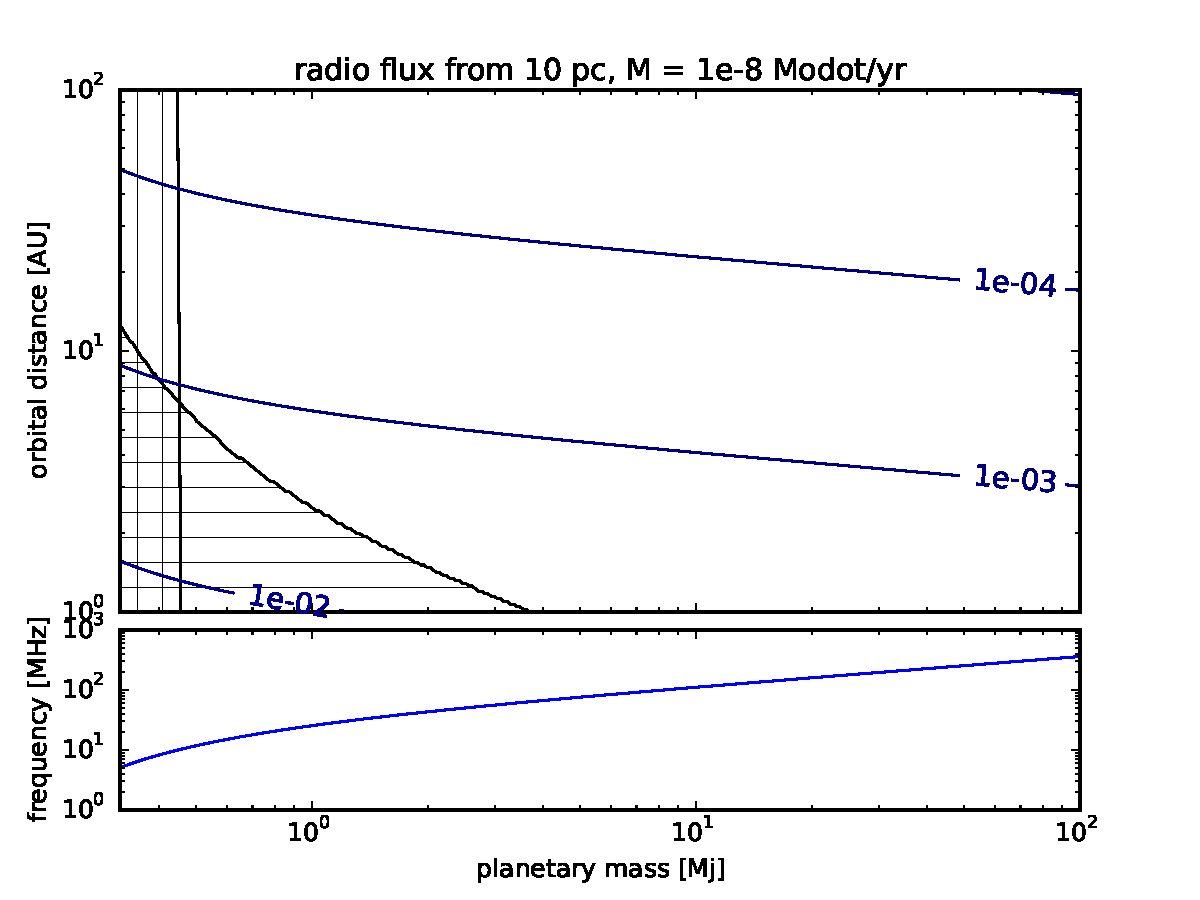
\includegraphics[width=\hsize]{radio_emission_Mdot1e-8_constRp.pdf}
%   \plotonesc{radio_emission_Mdot1e-8_constRp.eps}
  %\end{center}
 %\end{minipage}
 %\begin{minipage}{0.5\hsize}
   %\begin{center}
   %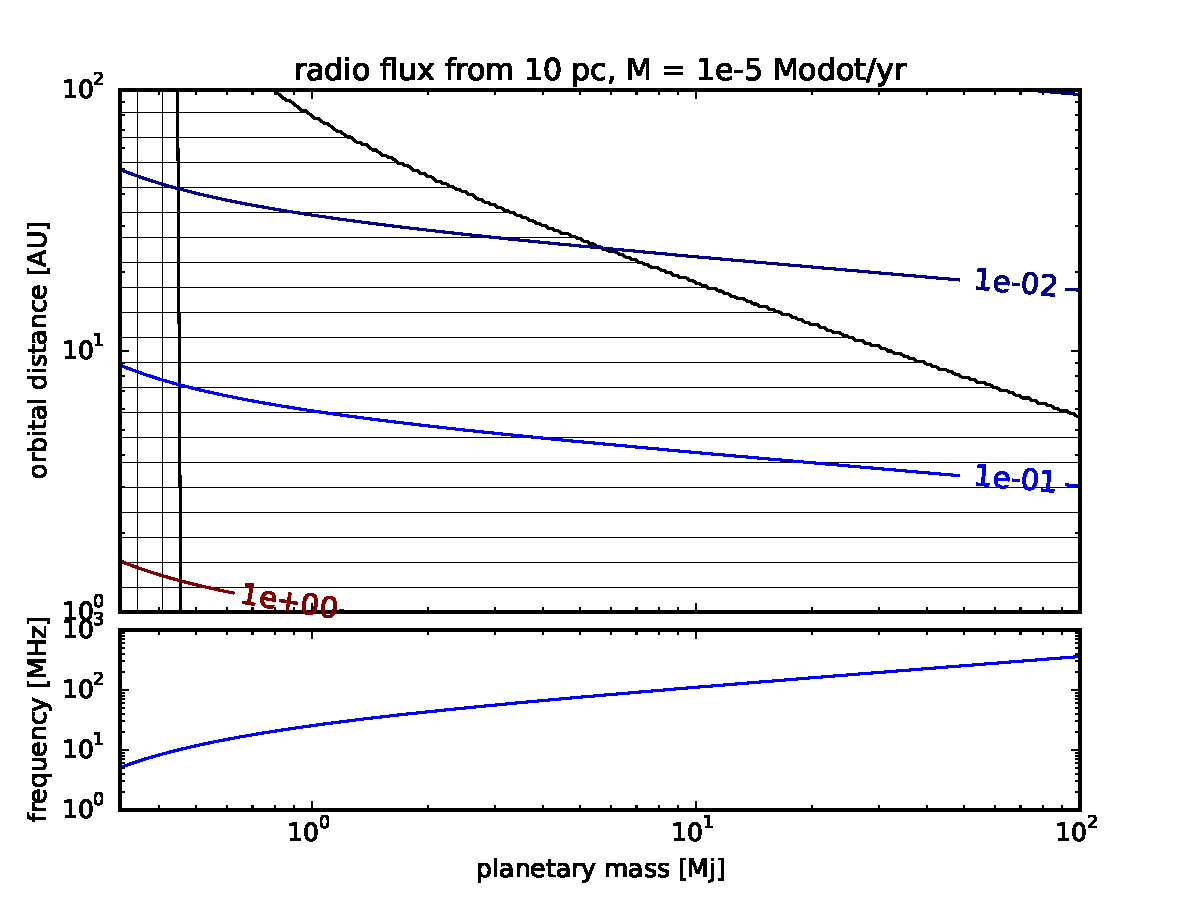
\includegraphics[width=\hsize]{radio_emission_Mdot1e-5_constRp.pdf}
%   \plotonesc{radio_emission_Mdot1e-5_constRp.eps}
  %\end{center} 
 %\end{minipage}
%   \caption{[{\bf Old version: based on scaling relationship of Sano 1993}] Top panel: Intensity of radio emission (in the unit of Jy) from a companion to a RG star (left) and an AGB star at 1 pc. The hashed region with vertical lines are not observable because of the plasma frequency cut-off of Earth's ionosphere. The hashed region with horizontal lines are not observable because of the plasma frequency cut-off of the stellar wind plasma in the vicinity of the companion. Bottom panel: cyclotron frequency, i.e., the frequency of radio emission. }
%  \label{fig:radio}
%\end{figure*}
%%%%%%%%%%%%%%%%%%%%%%%%%%%%%%%%%%%

%%%%%%%%%%%%%%%%%%%%%%%%%%%%%%%%%%%%%%%%%%%%%%%%%%%%%%%%%%%%%%%%%%%
\section{Observability}
\label{s:observability}
%%%%%%%%%%%%%%%%%%%%%%%%%%%%%%%%%%%%%%%%%%%%%%%%%%%%%%%%%%%%%%%%%%%


%%%%%%%%%%%%%%%%%%%%%%%%%%%%%%%%%%%
\begin{figure}[tbhp]
   \plotoneh{radio_1Mp_5AU.pdf}
%   \plotoneh{radio_5Mp_5AU.pdf}
   \plotoneh{radio_2Mp_4-5Gyr.pdf}
   \plotoneh{radio_4Mp_4-5Gyr.pdf}   
   \caption{Radio emission from existing M-type red giants with a hypothetical planetary companion of 1$M_J$, 2$M_J$, and 4$M_J$ at 1 AU and 5AU. Cross symbols indicate that the radio emission is not observable because cyclotron frequency is less than plasma density around the planet. }
  \label{fig:observability}
\end{figure}
%%%%%%%%%%%%%%%%%%%%%%%%%%%%%%%%%%% 

In order to examine the potential to detect radio emission of RGHJs with the current and near-future instruments, we estimate the possible radio emission from actual red giants in the case that they have planetary companions around them. 
For this purpose, we obtained the list of M-type red giants from Table 4 of \citet{dumm1998} with the values of mass, radius, and effective temperature, and also obtained the values of parallax from the original Hipparcos datasets\footnote{http://www.rssd.esa.int/index.php?project=HIPPARCOS} to compute thes distance.

For each red giant, the mass-loss rate is estimated by Reimers' equation \citep{reimers1975}:
%%%
\begin{equation}
\dot M_\star [M_\odot{\rm /yr}] \sim 4 \times 10^{-13} \left( \frac{R_{\star }}{R_{\odot }} \right)\left( \frac{L_{\star }}{L_{\odot }} \right) \left( \frac{M_\star}{M_\odot} \right)^{-1}
\end{equation}
%%%
where $R_{\star }$, $L_{\star } (=4\pi R_{\star }^2 T_{\star }^4)$, and $M_{\star}$ are radius, luminosity, and mass of the star. 
The velocity of stellar wind is assumed to scale with the escape velocity, hence
%%%
\begin{equation}
v \propto \sqrt{\frac{2GM_\star}{R_{\star }}}
\end{equation}
%%%
Using these values for equations (\ref{eq:stand-off}) and (\ref{eq:stand-off-radius}) as well as the distance to the target, we can estimate the frequency and intensity of radio emission by specifying planetary mass and orbital distance of a hypothetical planetary companion. 
Here, we consider [A] a Jupiter-twin whose cyclotron frequency is $\sim 30$~MHz, [B] a larger Jovian planet with $M_p\sim 2M_p$ of 4.5 Gyrs old whose cyclotron frequency is $\sim 70$~MHz, and [C] a larger Jovian planet with $M_p\sim 4M_p$ of 4.5 Gyrs old whose cyclotron frequency is $\sim 200$~MHz
  (equation (\ref{eq:scalingfc})).  

Figure \ref{fig:observability} displays the estimated radio intensity and the maximum frequency (i.e., cyclotron frequency) of Jupiters [A], [B], and [C]  around red giants within 100~pc. 
Jupiters are placed at 1 AU and at 5 AU for reference. 
The difference of the symbols indicates whether the radio emission can escape from the system (circle) or not (cross). 

%\memoYF{Up to where would the planet be engulfed by evolved stars? References?}
%I wondered this because if planets at 1 AU would be engulfed anyway it would not be worth discussing here. According to e.g. Nordhaus and Spiegel (2013) it is the case--however, some planets may migrate inward within 1 AU after evolution. So it should be ok. In any case this is not the main point of this paper and I would leave it out. 

\memoYF{discussion about detectability... Figures 1-3 of \citet{griesmeier2007b} show $10^{-3}$ Jy limit for 10-100 MHz (LWA, LOFAR) and $10^{-5}-10^{-4}$ Jy for 100-1000 MHz (LOFAR, SKA). }


%%%%%%%%%%%%%%%%%%%%%%%%%%%%%%%%%%%%%%%%%%%%%%%%%%%%%%%%%%%%%%%%%%%%%%%%
\newpage

%%%%%%%%%%%%%%%%%%%%%%%%%%%%%%%%%%%%%%%%%%%%%%%%%%%%%%%%%%%%%%%%%%%
\section{Discussions}
\label{s:discussion}
%%%%%%%%%%%%%%%%%%%%%%%%%%%%%%%%%%%%%%%%%%%%%%%%%%%%%%%%%%%%%%%%%%%

%%%%%%%%%%%%%%%%%%%%%%%%%%%%%%%%%%%%%%%%%%%%%%%%%%%%%%%%%%%%%%%%%%%
\subsection{Intrinsic radio emission of red giants stars}
\label{ss:RGradio}
%%%%%%%%%%%%%%%%%%%%%%%%%%%%%%%%%%%%%%%%%%%%%%%%%%%%%%%%%%%%%%%%%%%

(Jason?)

In the radio range, the brightness source of the radio emission is Rayleigh-Jeans tail of the Planck function, i.e., $S_{\nu } = 2kT\nu^2/c^2$. Recent observations revealed that this dependence on $\nu$ ($f \propto \nu^{\alpha }$ where $\alpha $ is 2) can approximately be extended as low frequency as 1 GHz \citep{gorman2013}, presumably as a result of the wavelength dependence of the opacity (at longer wavelength we see the region further from the center of the stars) and the decreased temperature as the distance from the stars increases. 
In this paper, we simply assume that the radio emission from the red giants themselves is approximated as a black body radiation at 1000~GHz and proportional to $\nu ^{5/3}$. 
Thus, the flux from the giants is:
%%%
\begin{eqnarray}
f_{\star } (\nu ) &=& \frac{2R_{\star }^2 k_B T \nu^2}{c^2 d^2}  \\
&\approx & 1.56 \times 10^{-6} ~\mbox{Jy} \left( \frac{d}{10 ~\mbox{pc}} \right)^{-2} \\
&& \times \left( \frac{R_{\star }}{10 R_{\odot }} \right)^2 \left( \frac{T_{\star }}{10^{4}~\mbox{K}} \right) \left( \frac{\nu}{1~\mbox{GHz}} \right)^{5/3} 
\end{eqnarray}
%%%
The brightest emission due to interaction with planetary companion to the RGB stars would therefore overwhelm the radio emission from their host stars in the 10-100~MHz range (in the 100-1000~MHz range) unless the stellar radius $R_{\star }$ is larger than $\sim 2000R_{\odot }$ ($\sim 300R_{\odot }$). 



\newpage


%%%%%%%%%%%%%%%%%%%%%%%%%%%%%%%%%%%%%%%%%%%%%%%%%%%%%%%%%%%%%%%%%%%
\subsection{Back-reaction of a plasma flowing into a magnetic field}
\label{ss:offset}
%%%%%%%%%%%%%%%%%%%%%%%%%%%%%%%%%%%%%%%%%%%%%%%%%%%%%%%%%%%%%%%%%%%

One might expect that plasma flowing into a region permeated by a magnetic field would, by spiraling around the field lines, generate an opposing magnetic field that partially cancels the intrinsic planetary magnetic field. 
To estimate the strength of this effect, consider a uniform flow of particles of charge $e$, mass $m$, and velocity $v$ into a region of magnetic field $B$, spiraling along the initial magnetic field. 
A single charged particle moving perpendicular to the magnetic field moves in a circular orbit of radius 
%%%
\begin{equation}
r=\frac{mv}{eB}.
\end{equation}
%%%
which creates a magnetic dipole
%%%
\begin{equation}
\mu = \frac{e}{2\pi r/v} \pi r^2 = \frac{1}{2} e r v = \frac{mv^2}{2B}.
\end{equation}
%%%
The volume integral of the canceling magnetic field $B_c$ generated by a single dipole $\mu$ is
%%%
\begin{equation}
\int d^3{\boldsymbol r} B_c = \frac{8\pi}{3} \mu.
\end{equation}
%%%

---

%%%
Hence, for a number density $n$ of these charged particles, the fraction of canceling field to the background magnetic field is
%%%
\begin{equation}
\frac{B_c}{B} = \frac{n(mv^2/2)}{3 B^2/8\pi}= \frac{\rho_K}{3\rho_B},
\end{equation}
%%%
where $\rho_K$ and $\rho_B$ are the kinetic energy density and the magnetic energy density, respectively. If the initial velocity is not perpendicular to the magnetic field, $v$ must everywhere be replaced by its perpendicular component.

%
At the magnetic stand-off point, 
%%%
\begin{equation}
m_p n[r_s] v^2 = \frac{B[r_s]^2}{2\pi }
\end{equation}
%%%
and thus $\rho_K \sim \rho _B$. When the particle spirals into the planet, the kinetic energy of the moment is
%%%
\begin{equation}
\frac{mv^2}{2} \propto \frac{1}{r}
\end{equation}
%%%
while magnetic pressures increases (by beaming?) by 
%%%
\begin{equation}
\frac{B^2}{8\pi } \propto \frac{1}{r^6}
\end{equation}
%%%
therefore, unless the density increases more drastically than $1/r^5$, the ratio $B_c/B$ is significantly less than unity. 

\memoYF{$\ast \ast \ast$ How about the following argument instead? $\ast \ast \ast$}

%%%
\begin{equation}
r=\frac{mv_{\bot }}{eB}.
\end{equation}
%%%
which creates a magnetic dipole
%%%
\begin{equation}
\mu = \frac{e}{2\pi r/v_{\bot }} \pi r^2 = \frac{1}{2} e r v_{\bot } = \frac{mv_{\bot }^2}{2B}.
\end{equation}
%%%
The volume integral of the canceling magnetic field $B_c$ generated by a single dipole $\mu$ is
%%%
\begin{equation}
\int d^3{\boldsymbol r} B_c = \frac{8\pi}{3} \mu.
\end{equation}
%%%

At the magnetic stand-off point, 
%%%
\begin{equation}
\left. \frac{B_c}{B}\right|_{r=r_s} = \frac{8\pi n \mu}{3B} = \frac{4\pi nmv_{\bot }^2}{3 B^2}
\end{equation}
%%%
but because
%%%
\begin{equation}
m_p n v^2 \sim \frac{B^2}{2\pi }
\end{equation}
%%%
and because $v_{\bot }^2 < v^2$, we have $|B_c/B| < 2/3$. 
When the particles are spiraling down along the magnetic field line, the magnetic dipole moment are approximately constant. 
On the other hand, the ambient magnetic field strength increase as $\propto r^{-3}$ where $r$ is the distance from the center of a planet. 


---

%Since by definition $\rho_K/\rho_B < 1$ inside the magnetic stand-off point where the auroral emission is from, the canceling magnetic field is much smaller than the canceling magnetic field. 

It is interesting to note that, for a plasma of protons and electrons in a stellar wind, the canceling field is clearly dominated by the contribution of protons, though the cyclotron emission is dominated by electrons. 


%%%%%%%%%%%%%%%%%%%%%%%%%%%%%%%%%%%%%%%%%%%%%%%%%%%%%%%%%%%%%%%%%%%%%%%%
\section{Conclusions}
\label{sec:conc}

In this paper, we propose that ``hot Jupiters'' around evolved stars (RGHJ) may be bright radio wave emitters, on the assumption of the simple empirical correlation between the radio emission and the kinetic input energy. 
Massive stellar wind of red giants and AGB stars would put the kinetic energy into magnetospheres of distant Jovian planets, which could lead to the intrinsic bright radio emission, which is comparable to or by far greater than canonical hot Jupiters in close-in orbits. 

The maximum radio emission we can expect to observe is limited by the plasma cut-off frequency of the stellar wind in the vicinity of the planets. 
For a planet with the same magnetic moment as Jupiter, the maximum radio emission from the planets which can penetrate through the surrounding plasma is $\sim 10^{-3}$ Jy or $\sim 10^{-5}$ Jy at 10 pc and 100 pc, respectively. 
\memoYF{comment on observability...}

Admittedly, uncertainties exist both in the scaling of planetary magnetic field  and the scaling of radio emission of Jovian planets in relation to the input energy. 
Alternatively, once we detect both the gravitational perturbation and radio emission of Jovian planets, these models will be contested. The viability of these scaling relations will be examined in the future. 

%The planetary magnetic moment is computed based on the simple scaling relationship given by \citep{christensen2010}. 
%-about detectability
%-number of evolved stars within 100pc $\sim 1000$. 

\vspace{0.5in}

\acknowledgements

{\sc Acknowledgments}

YF is supported from the Grant-in-Aid No. 25887024 by the Japan Society for the Promotion of Science.
DSS gratefully acknowledges support from a fellowship from the AMIAS group.
We thank David Hogg for encouraging us to pursue calculations of explanetary radio emission.
NM acknowledges support from [???].


\bibliography{biblio.bib}


\clearpage

%\end{document}



\section{Memo}

%%%%%%%%%%%%%%%%%%%%%%%%%%%%%%%%%%%%%%%%%%%%%%%%%%%%%%%%%%%%%%%%%%%
\subsection{Brighter Implies Harder to See:\\
Greater $B$ Produces Lower $F_\nu$}
\label{ss:counterintuitive}
%%%%%%%%%%%%%%%%%%%%%%%%%%%%%%%%%%%%%%%%%%%%%%%%%%%%%%%%%%%%%%%%%%%


The cyclotron frequency at radius $r$ is:
%%%
\begin{equation}
f_{\rm cyc} = \frac{e B(r)}{2\pi m_e} \propto \frac{B_p}{r^3}
\end{equation}
%%
Therefore, 
%%%
\begin{equation}
\frac{dP}{df_{\rm cyc}} = \frac{dP}{d\nu } \propto -\frac{r^4}{B_p} \frac{dP}{dr}
\end{equation}
%%%
Employing Larmor formula, power emitted from a thin shell at $r\sim r+dr$, $dP/dr$ is 
%%%
\begin{equation}
\frac{dP}{dr} \propto 4\pi r^2 N_{\rm plasma}(r) v_{\bot }^2(r) B^2(r) \label{eq:larmor}
\end{equation}
%%%
where $N_{\rm plasma}(r) $ represents the number density of plasma in the planetary magnetosphere at radius $r$. 

We assume that $N_{\rm plasma}(r_s) $  is proportional to the squared radius of the magnetic stand-off point:
%%%
\begin{equation}
N_{\rm plasma}(r_s) \propto \pi r_s^2 \;\;(\propto B_p^{2/3}) \label{eq:N0_plasma}
\end{equation}
%%%
Due the the mass flux conservation,
%%%
\begin{equation}
4 \pi r^2 N_{\rm plasma}(r) v_{\|} = const.
\end{equation}
%%%
Combining with equation (\ref{eq:N0_plasma}),
%%%
\begin{equation}
N_{\rm plasma}(r) \propto  \frac{r_s^2 }{v_{\|}(r) r^2} \propto  B_p^{2/3} \cdot \frac{v_{\|}(r)}{r^2}
\end{equation}
%%%

Because the magnetic dipole moment
%%%
\begin{equation}
\mu = \frac{mv_{\bot}(r)}{eB(r)}
\end{equation}
%%%
is approximately to be constant while the plasma falls down along the magnetic field, 
%%%
\begin{eqnarray}
v_{\bot }(r) \propto \frac{1}{r^3} \label{eq:v_bot} \\
B(r) \propto \frac{B_p}{r^3} 
\end{eqnarray}
%%%
On the other hand, conservation of energy ensures that
%%%
\begin{equation}
\mathcal{E} = -\frac{GM_p}{r} + \frac{v_{\bot }^2}{2} + \frac{v_{\|}^2}{2}=const.
\end{equation}
%%%
Assuming that the initial energy (at $r=r_s$) is negligible compared to those near the surface, $\mathcal{E}=0$, 
%%%
\begin{equation}
v_{\|}^2 \sim \frac{GM_p}{r} - \frac{v_{\bot ,0}^2}{2} \left( \frac{r}{r_s} \right)^{-6} \label{eq:v_||}
\end{equation}
%%%

Substituting equations (\ref{eq:N0_plasma}),  (\ref{eq:v_bot}) and (\ref{eq:v_||}) into equation (\ref{eq:larmor}) leads to
%%%
\begin{equation}
\frac{dP}{dr} \propto \frac{B_p^{8/3}}{r^{12}} \left( \frac{GM_p}{r} - \frac{v_{\bot ,0}^2}{2} \left( \frac{r}{r_s} \right)^{-6} \right)^{1/2}  
\end{equation}
%%%
The right-hand side has the maximum value $\sqrt{5GM_p/6\tilde r} $ at radius $\tilde r=(6v_{\bot ,0}^2/GM_p)^{1/5}$. 
At $r>>\tilde r$, 
%%%
\begin{equation}
\frac{dP}{dr} \propto \frac{B_p^{8/3}}{r^{25/2}}
\end{equation}
%%%
and
%%%
\begin{equation}
\frac{dP}{d\nu } \propto \frac{B_p^{5/3}}{r^{17/2}} \propto \frac{\nu^{17/6}}{B_p^{7/6}}
\end{equation}
%%%


At $r<<\tilde r$, 
%%%
\begin{equation}
\frac{dP}{dr} \propto \frac{B_p^{8/3}}{r^{15}}
\end{equation}
%%%
and
%%%
\begin{equation}
\frac{dP}{d\nu } \propto \frac{B_p^{5/3}}{r^{11}} \propto \frac{\nu^{11}}{B_p^{28/3}}
\end{equation}
%%%




\newpage







\memoDS{Is this section needed anymore, since this is already in the Griesmeier paper?
Does the Griesmeier paper make the point explicit enough, or is this still somewhat valuable?
Also, are we 100\% sure that this section is right?
A planet with larger surface field achieves an equivalent field to a planet with a smaller surface field at a larger radius, and captures a larger wind flux.
Should we think more about the spectrum?}





According to Eq.~(\ref{eq:Pkinp}), the total emitted power scales with $B^{2/3}$.
In detail, it is not obvious how the power spectral density scales with a planet's surface magnetic field, because the emission process involves electrons passing through a wide range of magnetic field conditions (dipolar field strength drops off as $r^{-3}$, and only in an idealized model is a planet a perfect magnetic dipole).
Nevertheless, a reasonable ansatz is that the radio emission is spread over a range of wavelengths in an approximately scale-independent way.
In other words, the frequency bandwidth $\Delta f$ of Eq.~(\ref{eq:Fnu}) is proportional to $f_{\rm cyc}$, as described in Section~\ref{ss:model_intensity} and in \citet{griesmeier2007b}.
This means that the power spectral density is likely to scale as the total power divided by the cyclotron frequency corresponding to a characteristic field strength where the emission peaks.
Since $f_{\rm cyc}$ scales as $B$ (a higher power of $B$ than the scaling of total power), this implies that the power spectral density in the radio scales as $B^{-1/3}$.
Planets that are intrinsically brighter, owing to a greater magnetic field strength, probably have their emission spread out over a broader set of frequencies, and therefore have a lower flux density as measured in Janskys!
\memoDS{Is this pointed out elsewhere in the literature?}



\section{Dave's sketch}

\citep{spiegel2008}

\citep{lecavelier_et_al2013}

\citep{janhunen_et_al2003}

\citep{zarka1992, zarka1998}

\citep{farrell_et_al2004}

\citep{lazio+farrell2007}: likelihood function, tau Boo search

\citep{lecavelier_et_al2009}

\citep{spiegel2012}

\citep{nordhaus+spiegel2013}



\citep{jiang+jin1996}: 12cm radio of Jupiter during Shoemake-Levy-9

\citep{morin2012, morin_et_al2013}

\citep{christensen_et_al2009, christensen2010}

\citep{saar2001}: Inverse rossby number scaling of magnetic field: $B
\sim 60 {\rm~G} \times Ro^{-1.2}$.  Here, he takes $Ro = \tau_c/P_{\rm
  rot}$, where $\tau_c$ is the convective turnover time = ?
\citep{gilliland1986}.  Well, $F \sim \rho v_c^3 \sim \rho
(H/\tau_c)^3$, so $\tau_c \sim H (\rho / F)^{1/3} = H / (\sigma T_{\rm
  eff}^4 / \rho)^{1/3}$.  Alternatively, $\tau_{\rm conv} \sim (M R^2
/ L)^{1/3}$.

On dimensional grounds, the convective turnover time goes as
$\tau_{\rm conv} \sim (M R^2 / L)^{1/3}$.  According to
\citet{burrows_et_al2001}, radius $R$ and luminosity scale with time
as $R \sim R_J$, where $R_J$ is the radius of Jupiter, and
\begin{equation}
\frac{L}{10^{-9} L_\odot} \sim \left( \frac{t}{1 \rm~Gyr} \right)^{-1.3} \left( \frac{M}{1~M_J} \right)^{2.64} \, .
\label{eq:burrowsLum_2}
\end{equation}
So,
%\begin{eqnarray}
%\nonumber \tau_{\rm conv} & \sim & 3 {\rm~days} \times \left( \frac{M}{M_J} \right)^{1/3} \left( \frac{R}{R_J} \right)^{2/3} \left( \frac{L}{L_\odot} \right)^{-1/3} \\
% & = & 
%\end{eqnarray}
\begin{eqnarray}
\nonumber \tau_c & \sim & 3 {\rm~hrs} \times \frac{\left( \frac{H}{100 \rm~km} \right) \left( \frac{\rho}{10^{-5} \rm~g~cm^{-3}} \right)^{1/3}}{\left( \frac{L}{10^{-9} L_\odot} \right)^{1/3}} \\
 & = & 3 {\rm~hrs} \times \frac{\left( \frac{H}{100 \rm~km} \right) \left( \frac{\rho}{10^{-5} \rm~g~cm^{-3}} \right)^{1/3}}{\left( \frac{M}{1 ~M_J} \right)^{0.88} \left( \frac{t}{1 \rm~Gyr} \right)^{0.43}} \\
\end{eqnarray}
So the Rossby number $Ro = \tau_c/P_{\rm rot}$ is
\begin{eqnarray}
Ro & = & \frac{\tau_c}{P_{\rm rot}} \\
 & = & \left( \frac{P_{\rm rot}}{3 \rm~hrs} \right)^{-1} \times \frac{\left( \frac{H}{100 \rm~km} \right) \left( \frac{\rho}{10^{-5} \rm~g~cm^{-3}} \right)^{1/3}}{\left( \frac{M}{1 ~M_J} \right)^{0.88} \left( \frac{t}{1 \rm~Gyr} \right)^{0.43}}
\end{eqnarray}

\citep{hallinan_et_al2013}

\citep{desch+kaiser1984} radiometric Bode's law

Noting that
\begin{equation}
\dot{M}_* = 4\pi r^2 \rho[r] v \, ,
\label{eq:mdot}
\end{equation}
so $\rho[r] = \dot{M}_*/(4\pi r^2 v)$,
\begin{eqnarray}
\frac{\rho v^2}{2} = \frac{B^2}{8\pi} \sim \frac{B_0^2}{8\pi} \left( \frac{d}{d_0} \right)^{-3} \, ,
\end{eqnarray}
where $B_0$ is the field strength at a distance $d_0$ from the planet.
\begin{eqnarray}
\frac{\rho v^2}{2} & \sim & \frac{B_0^2}{8\pi} \left( \frac{d}{d_0} \right)^{-6} \\
\frac{\dot{M}_* v}{8\pi a^2} & = & \frac{B_0^2}{8\pi} \left( \frac{d}{d_0} \right)^{-6} \\
\frac{\dot{M}_* v}{r^2} & = & B_0^2 \left( \frac{d}{d_0} \right)^{-6} \\
d^6 & = & \frac{d_0^6 B_0^2 r^2}{\dot{M}_* v} \\
d_A & = & d_0 \left( \frac{B_0^2 r^2}{\dot{M}_* v} \right)^{1/6} \\
  & \sim & 4 R_J \left( \frac{d_0}{R_J}\right) \left\{ \frac{\left( \frac{B}{10 \rm~G} \right)^2 \left( \frac{r}{5 \rm~AU} \right)^2}{\left( \frac{\dot{M}_*}{10^{-6} M_\odot/\rm yr} \right) \left( \frac{v}{20 \rm~km/s} \right)} \right\}^{1/6}
\label{eq:Chapman-Ferraro}
\end{eqnarray}
In the above, $d_A$ is the distance from the planet to the Alfven
point, where the magnetic energy density $u_B = B^2 / 8\pi$ equals the
kinetic energy density in the stellar wind $u_w = \rho v^2/2$, and
$B_0$ is the magnetic field strength at distance $d_0$.

The escape speed is
\begin{equation}
v_{\rm esc}^* = \sqrt{\frac{2 G M_*}{R_*}} \, ,
\end{equation}
so if the stellar wind speed is a factor $C$ times the escape speed, then ...

The power incident on the planet within $d_A$ is
\begin{eqnarray}
P_{\rm inc} & = & \frac{\rho v^3}{2} \times \pi d_A^2 \\
\frac{\rho v^2}{2} & \sim & \frac{B_0^2}{8\pi} \left( \frac{d}{d_0} \right)^{-6} \\
d_A^6 & = & d_0^6 \frac{B_0^2}{4\pi \rho v^2} \\
d_A^2 & = & d_0^2 \left( \frac{B_0^2}{4\pi \rho v^2}\right)^{1/3} \\
\pi d_A^2 \frac{\rho v^3}{2} & = & \frac{d_0^2}{2} \left( \frac{\pi^2 \rho^2 v^7 B_0^2}{4} \right)^{1/3} \\
P_{\rm inc} & = & d_0^2 \left( \frac{\pi^2 \rho^2 v^7 B_0^2}{32} \right)^{1/3} 
%\frac{\dot{M}_* v}{8\pi a^2} & = & \frac{B_0^2}{8\pi} \left( \frac{d}{d_0} \right)^{-6} \\
%\frac{\dot{M}_* v}{r^2} & = & B_0^2 \left( \frac{d}{d_0} \right)^{-6} \\
%d^6 & = & \frac{d_0^6 B_0^2 r^2}{\dot{M}_* v} \\
%d_A & = & d_0 \left( \frac{B_0^2 r^2}{\dot{M}_* v} \right)^{1/6} \\
%  & \sim & 4 d_0 \left\{ \frac{\left( \frac{B}{10 \rm~G} \right)^2 \left( \frac{r}{5 \rm~AU} \right)^2}{\left( \frac{\dot{M}_*}{10^{-6} M_\odot/\rm yr} \right) \left( \frac{v}{20 \rm~km/s} \right)} \right\}^{1/6}
\end{eqnarray}
Note that $\rho v = \dot{M}_*/4\pi r^2$.  Therefore,
\begin{eqnarray}
P_{\rm inc} & = & d_0^2 \left( \frac{\pi^2 \rho^2 v^7 B_0^2}{32} \right)^{1/3} \\
 & = & d_0^2 \left( \frac{\dot{M}_*^2 v^5 B_0^2}{512 r^4} \right)^{1/3} \\
 & = & \frac{d_0^2}{8} \left( \frac{\dot{M}_*^2 v^5 B_0^2}{r^4} \right)^{1/3} \\
\nonumber  & \sim & 2 \times 10^{18} {\rm~W} \left( \frac{d_0}{R_J} \right)^2 \left( \frac{\dot{M}_*}{10^{-5} M_\odot / {\rm yr}} \right)^2 \\
 & & \times \left( \frac{v}{20 \rm~km/s} \right)^5 \left( \frac{B_0}{10 \rm~G} \right)^2 \left( \frac{r}{5 \rm~AU} \right)^{-4}
\end{eqnarray}


The power incident on the planet is

%\citep{lunine_et_al1989} -- error?

% http://kiss.caltech.edu/workshops/magnetic2013/presentations/winterhalter.pdf

%ftp://ftp.iwf.oeaw.ac.at/pub/Scherf/PRE-CD%20V2/pre6/nigl.pdf

%%%%%%%%%%%%%%%%%%%%%%%%%%%%%%%%%%%%%%%%%%%%%%%%%%%%%%%%%%%%%%%%%%%
\subsection{Assumptions for Planetary Magnetic Field}
%\label{ss:magneticfield}
%%%%%%%%%%%%%%%%%%%%%%%%%%%%%%%%%%%%%%%%%%%%%%%%%%%%%%%%%%%%%%%%%%%

\memoYF{It may be better to consider Cristensen's scaling, taking account of the age. But I have not followed the theory yet.}

Theoretically, the magnetic moment of gaseous planets are expressed with the following scaling relationship \citep{griesmeier2004}:
%%%%%%%%%% 
\begin{equation}
\mathcal{M} \propto  \omega ^{\alpha } \rho_c ^{\beta } r_c^{\gamma } \sigma ^{\delta }
\end{equation}
%%%%%%%%%%
where $\omega $ is the spin angular velocity, $\rho _c$, $r_c$ and $\sigma $ are the density, the radius, and the conductivity of the ``dynamo region'' where the density is high enough for hydrogen to be metallic, respectively. 
The scaling indexes are estimated to be $\alpha \sim 1/2-1$, $\beta \sim 1/2$, $\gamma \sim 3-4$, and $\sigma \sim -1/2-0$. In this paper, we assume $\alpha =1$, $\beta =1/2$, and $r_c = 7/2$ \citep{sano1993}. \memoYF{validity?}

Unlike usual hot jupiters, RGHJs are not subject to tidal lock, as the gravitational effects of their host star does not change even if the star evolves into red giants. Without no physical insights of the typical spin rate, we simply assume that of Jupiter: $\omega = 9.925$ [hr]. 
\memoYF{Would their spin rate become higher or lower??}

In order to evaluate $\rho _c $ and $r_c$, we need a model of internal structure of gaseous planets. 
First, we assume that the planetary radius is constant at $R_p = R_{p,J}$, as the numerical calculations show that the radii of gaseous planets over the range of $0.1 R_{p, J} < M_p < 10M_{p, J}$ (with core mass less than 10\%) are converged to $0.8 R_{p, J} < R_p < 1.2R_{p, J}$ in 1 Gyr \citep{fortney2007}. 
For the density profile, we assume a polytrope gas sphere with index $n=1$, which results in:
%%%%%%%%%% 
\begin{equation}
\rho [r] = \left( \frac{\pi M_p}{4 R_p^3} \right) \frac{\sin \left[ \pi \frac{r}{R_p} \right]}{\left( \pi \frac{r}{R_p} \right)}. \label{eq:rho_r_2}
\end{equation}
%%%%%%%%%%
We determine the core radius $r_c$ by assuming that the hydrogen becomes metallic when $\rho (r)$ exceeds the critical density $\rho_c=700\,\mbox{kg/m}^3$. The density of the metallic core, $\rho _c$ is obtained by averaging the density in the core. 
We assume that the conductivity $\sigma $ is the same as Jupiter \memoYF{?}. 




\end{document}

